%!TEX root = thesis.tex
\chapter{Model implementation}\label{chap:methods}
\thispagestyle{plain}

% ==== SECTION 1 ===============================================================
\section{General concepts} % (fold)
\label{sec:general_concepts}

    \subsection{Glacier volume/area scaling} % (fold)
    \label{sub:glacier_volume_area_scaling}

        % Overview

        % Physical basis, from two independet methods, ...

        % Drawbacks
    
    % subsection glacier_volume_area_scaling (end)

    \subsection{Temperature index model} % (fold)
    \label{sub:temperature_index_model}

        In a nutshell, a glaciers annual specific surface mass balance $B$ is the difference between accumulation and over the course of a year. Hereby, accumulation refers to mass gain by snowfall, avalanches, snow drift, etc., while ablation refers to mass loss via ice melt, sublimation, calving, etc. The temperature index mass balance model used by the \vas{} model relies solely on the area average monthly solid precipitation onto the glacier surface $P_i^\text{solid}$ and the monthly mean air temperature at the glacier's terminus elevation $T_i^\text{terminus}$ as input. Hereby, the index $i$ denotes the month of the year. The mass balance equation described by \citet{Marzeion2012b} reads
        \begin{align}
            \label{eq:mass-balance}
            B = \left[\sum_{i=1}^{12}\left[
                    P_i^\text{solid}  - \mu^* \cdot \max\left(T_{i}^\text{terminus} - T_\text{melt},\ 0\right)
                \right]\right] - \beta^*.
        \end{align}
        The terminus temperature $T_{i}^\text{terminus}$ is computed by scaling the monthly average air temperature $T_i$ from the climate file reference elevation $z_\text{ref}$ to the glacier's terminus elevation $z_\text{min}$ using the temperature lapse rate $\gamma_\text{temp}$.
        \begin{align}
            T_i^\text{terminus} = T_i \cdot \gamma_\text{temp} (z_\text{min} - z_\text{ref})
        \end{align}
        The temperature at the maximum glacier elevation $T_{i}^\text{max}$ is computed analogously to terminus temperature: $T_{i}^\text{max} = T_i \cdot \gamma_\text{temp} (z_\text{max} - z_\text{ref})$, whereby $z_\text{max}$ represent the maximum glacier surface elevation. The positive melting temperature is computed as the difference between terminus temperature and temperature threshold for ice melt $T_\text{melt}$, with an obvious lower bound of \SI{0}{\celsius}. The glacier's temperature sensitivity \mustar{} relates the positive melting temperature to the actual ice loss and needs to be calibrated for each glacier (as does the potential mass balance residual \bias{}). The \hyperref[ssub:mb_calib]{calibration process} of these mass balance parameters is described below.
        
        The area average monthly solid precipitation onto the glacier surface $P_i^\text{solid}$ is computed from the total precipitation $P_i$ (given by the climate file) as
        \begin{align}\label{eq:solid-precip}
            P_i^\text{solid} = P_i \cdot f_\text{solid} \cdot (1 + \gamma_\text{precip} \cdot (z_\text{mean} - z_\text{ref})).
        \end{align}
        The total climatic precipitation $P_i$ is scaled from the reference elevation of the climate file $z_\text{ref}$ to the average glacier surface elevation $z_\text{mean}$ using the precipitation lapse rate $\gamma_\text{precip}$. The precipitation lapse rate $\gamma_\text{precip}$ is given in percentage of precipitation per meters of elevation change [\si{\percent\per\meter}]. The fraction of solid precipitation $f_\text{solid}$ depends on the terminus temperature $T_i^\text{terminus}$, the temperature at the maximum glacier surface elevation $T_i^\text{max}$ and the temperature thresholds for solid and liquid precipitation, $T^\text{solid}$ and $T^\text{liquid}$, respectively. For terminus temperatures below the threshold for solid precipitation, all precipitation is solid ($T_i^\text{terminus} < T^\text{solid} \ \Rightarrow f_\text{solid} = 1$). For temperatures at the maximum glacier surface elevation above the threshold for liquid precipitation, all precipitation is liquid ($T_i^\text{max} > T^\text{liquid} \Rightarrow f_\text{solid} = 0$). For temperatures in between, the fraction of solid precipitation is interpolated linearly as $f_\text{solid} = 1 + \frac{T_{i}^\text{terminus} - T^\text{solid}}{\gamma_\text{temp}\cdot(z_\text{max} - z_\text{min})}$.
        
        Climate models generally tend to underestimate the precipitation in mountainous regions, hence the monthly precipitation amount is additionally scaled by a factor $a$. While this scaling factor is implemented in the mass balance models (as \lstinline`prcp_scaling_factor`), it is not a physical component of the  mass balance equation and hence omitted in the Equation~\ref{eq:solid-precip} above. A global mean of $a = 2.5$ is found by \citet{Giesen2012}, whereas \citet{Marzeion2012c} found a mean of 2.1 for Central Europe and Scandinavia. The sensitivity study by \citet{Marzeion2012b} shows the strongest correlation between observed and modeled mass balance for $a \approx 1.3$ and the highest skill score for $a \approx 2.5$. The variability of the modeled mass-balance is quite low for values of $a \leq 2.5$.

        The values of the above mentioned hyper parameters (temperature thresholds, lapse rates, scaling factors, ...) can be calibrated, depending on the region and the used baseline climate. For Alpine model runs with the HISTALP baseline climate the following values are recommended (set as default in OGGM) and used this work \citep{Dusch2018}: $\gamma_\text{temp} = \SI{-6.5}{\kelvin\per\kilo\meter}$, $T^\text{melt} = \SI{-1.75}{\celsius}$, $\gamma_\text{precip} = 0$, $T^\text{solid} = \SI{0.0}{\celsius}$, $T^\text{liquid} = \SI{2.0}{\celsius}$, $a = 1.75$;

        \subsubsection{Calibration of the mass balance parameters} % fold
        \label{ssub:mb_calib}

            A complete and thorough description of the mass balance calibration process for this particular temperature index model can be found in \citet[Section 2.1.9, 2.1.10]{Marzeion2012b} and \citet[][Section 3.3]{Maussion2019}. The following section serves as a summary.
            
            The first step is to estimate the so called \emph{candidates} $\mu(t)$ for all glaciers with available mass balance records (254 glaciers globally, see \citet{WGMS2017}). This is done by requiring the average mass balance $\overline B(t)$ over the 31-year period centered around the year $t$ to be zero and solving for $\mu(t)$.
            \begin{align}\label{eq:mu-candidates}
                \mu(t) = \frac{P_\text{clim}^\text{solid}(t)}{\max(T_\text{clim}^\text{terminus(t)} - T_\text{melt}\, 0)},
            \end{align}
            whereby $P_{\text{clim}}^{\text{solid}}(t)$ and $T_{\text{clim}}^{\text{terminus}}(t)$ are the average yearly solid precipitation amount and average yearly air temperature at the glaciers terminus during the climatological period centered around the year $t$, respectively. The next step is to solve the mass balance equation (Eq.~\ref{eq:mass-balance}) for each candidate $\mu(t)$ and compare it to the mass balance observations. The computed difference $\beta(t)$ is a measure of how good the temperature sensitivity candidate $\mu(t)$ approximates the \textit{real} value of \mustar{}. Hence, \mustar{} is chosen as the candidate $\mu(t = t^*)$ for which the absolute bias is minimal $\beta^* \coloneqq \beta(t = t^*) \approx 0$, which in the best case is around zero. Hereby, the \textit{equilibrium year} \tstar{} represents the center of a 31-year climatic period where the given glacier geometry would stay in equilibrium. However, this is more of a model parameter and should not be overinterpreted as a real live value. The same is true for the corresponding temperature sensitivity \mustar{} and mass balance residual \bias{}.

            For all glaciers without mass balance records, \tstar{} and \bias{} are interpolated from the ten closest glaciers, inversely weighted with distance. The temperature sensitivity is computed by requiring the mass balance to be zero $\overline B(t^*) = 0$ and solving for \mustar{}. The temperature sensitivity \mustar{} depends highly on glacier specific factors, such as avalanches from surrounding terrain, topographical shading, etc. Therefore, \mustar{} can vary drastically from one glacier to another, even between neighboring glaciers. On the other hand, it is intuitively more likely for a glacier to be in equilibrium if its surrounding glaciers are in equilibrium as well. This is one major factor, why the interpolation of \tstar{} instead of \mustar{} reduces the mass balance error in a leave--one--out cross--validation \citep[cf.][]{Marzeion2012b, Maussion2019}.

        % subsubsection mb_calib (end) 


        \subsubsection{Implementation note} % (fold)
        \label{ssub:mb_calib_implementation_note}

            The results of the steps above depend on the glacier outlines, the climate data and the mass balance hyper parameters (i.e., the temperature thresholds, lapse rates and the precipitation scaling factor). The equilibrium year \tstar{} and mass balance residual \bias{} computed for each reference glacier is stored in the \lstinline`ref_tstars.csv` file. Hence, for a given combination of RGI version, climate data and hyper parameters the calibration for the reference glaciers has to be done only once. Afterwards, it can be read directly from the corresponding file. OGGM comes with reference tables for combinations of RGI v5 and v6 and CRU4 and HISTALP.
        
        % subsubsection mb_calib_implementation_note (end) 

        \subsubsection{Differences between the flowline mass balance model and the \vas{} mass balance model}

            The \vas{} mass balance model computes an average mass balance value for the entire glacier. The mass balance model requires only the minimal and maximal glacier elevation as additional input parameters ($z_\text{min}$, $z_\text{max}$), to compute the monthly terminus temperature $T_i^\text{termiuns}$ and the area averaged monthly amount of solid precipitation $P_i^\text{solid}$. The flowline model, on the other hand, requires a mass balance value for each grid point of the flowline (i.e., for each elevation band). Therefore, the mass balance is a function of elevation $B(z)$ and the elevation of the grid points must be supplied. Solid precipitation and air temperature are then computed for the given points of elevation, resulting in a point mass balance.
    
    % subsection temperature_index_model (end)

    \subsection{Glacier evolution model} % (fold)
    \label{sub:glacier_evolution_model}

        % Volume/area scaling must be used in conjuncture with proper response time scaling (Bahr, 2015)
        \Vas{} is derived from the full set of continuum equations with no assumptions of plane strain, shallow ice, perfect plasticity, or steady state conditions. This derivation from the fully time dependent equation of motion allows the volume $V$, area $A$ and scaling constant $c_A$ to change with time. Especially the scaling constant $c_A$ can incorporate transient behavior, since it depends on closing conditions which show an explicit time dependency. However, to explicitly include a temporal component, \vas{} has to be used in conjuncture with proper response time scaling. Response time scaling is a separate but equally valid scaling relation, derived during the same dimensionless analysis. Hence, these two scaling relations cannot be separated and have to be applied together to successfully model glacier evolution \citep{Bahr2015}.

        % Initialization: start with area, compute volume and length from scaling relations
        The \vas{} model starts with an initial glacier surface area $A_0$ as input. The initial glacier volume $V_0$ and the initial glacier length $L_0$ are computed using the \vas{} relation and the inverted volume/length scaling relation, respectively (cf. Section~\ref{sub:glacier_volume_area_scaling}).
        \begin{align}
            \begin{split}
                V_0 = c_A\cdot A_0^\gamma \qquad\qquad L_0 = \left(\frac{V_0}{c_L}\right)^\frac{1}{q}
            \end{split}
        \end{align}
        Additionally, only a mass balance model and the initial terminus elevation $z_{\text{min},0}$ and maximal glacier surface elevation $z_\text{max}$ are needed.

        % Yearly steps
        The \vas{} model runs with yearly time steps $\Delta t = \SI{1}{\year}$. Each time step from year $t$ to year $t+1$ includes the following steps:
        \begin{enumerate}
            \item Compute the time scale of the glacier's length change response to volume change $\tau_L$ and the time scale of the glacier's surface area change response to volume change $\tau_A$ as
            \begin{align}
                \begin{split}
                    \tau_L(t) = \frac{V(t)}{P^\text{solid}_\text{clim}(t^*)\cdot A(t)}
                    \qquad\qquad
                    \tau_A(t) = \tau_L(t)\frac{A(t)}{L(t)^2}
                \end{split}
            \end{align}
            As introduced during the calibration process, $P^\text{solid}_\text{clim}(t^*)$ is the average solid precipitation during the 31-year period centered around \tstar{}. For more details see \citet{Marzeion2012b}. The implementation includes lower bounds for both time scales as well as the climatological turnover, for details see Section~\ref{sub:glacier_evolution_model_implementation}.
            \item Get the specific mass balance $B(t)$ from mass balance model, by solving Equation~\ref{eq:mass-balance}. For implementation details see Section~\ref{sub:mass_balance_models_implementation}
            \item Compute the volume change $\Delta V(t) = \frac{1}{\rho_\text{ice}}A(t)\cdot B(t)$ as product of specific mass balance and glacier surface area. The volume change happens instantaneously, i.e., over one time step, hence the updated volume equals the sum of current volume and volume change $V(t+1) = V(t) + \Delta V(t)$.
            \item The (hypothetical) equilibrium surface area can be computed by inverting the \vas{} relation $(V(t+1)/c_A)^{1/\gamma}$. However, the surface area does not change instantaneously, and proper response time scaling must be applied. Hence, the area change is computed as
            \begin{align}
                \Delta A(t) = \frac{1}{\tau_A}\left(\left(\frac{V(t+1)}{c_A}\right)^\frac{1}{\gamma} - A(t)\right).
            \end{align}
            The updated area then equals the sum of current area and area change $A(t+1) = A(t) + \Delta A(t)$.
            \item The updated glacier length and length change are computed analogously to the glacier surface elevation. $L(t+1) = L(t) + \Delta L(t)$, with
            \begin{align}
                \Delta L(t) = \frac{1}{\tau_L}\left(\left(\frac{V(t+1)}{c_L}\right)^\frac{1}{q} - L(t)\right).
            \end{align}
            \item Adjust terminus elevation $z_\text{min}$, assuming a linear elevation change with changing glacier length (i.e., constant slope):
            \begin{align}
                z_\text{min}(t+1) = z_\text{max} + \frac{L(t)}{L_0}(z_{\text{min},0} - z_\text{max})
            \end{align}
            The maximum glacier elevation stays constant during the entire model run $z_\text{max} = \text{const.}$
            
        \end{enumerate}
        
        \begin{figure}[tbh]
            \centering
            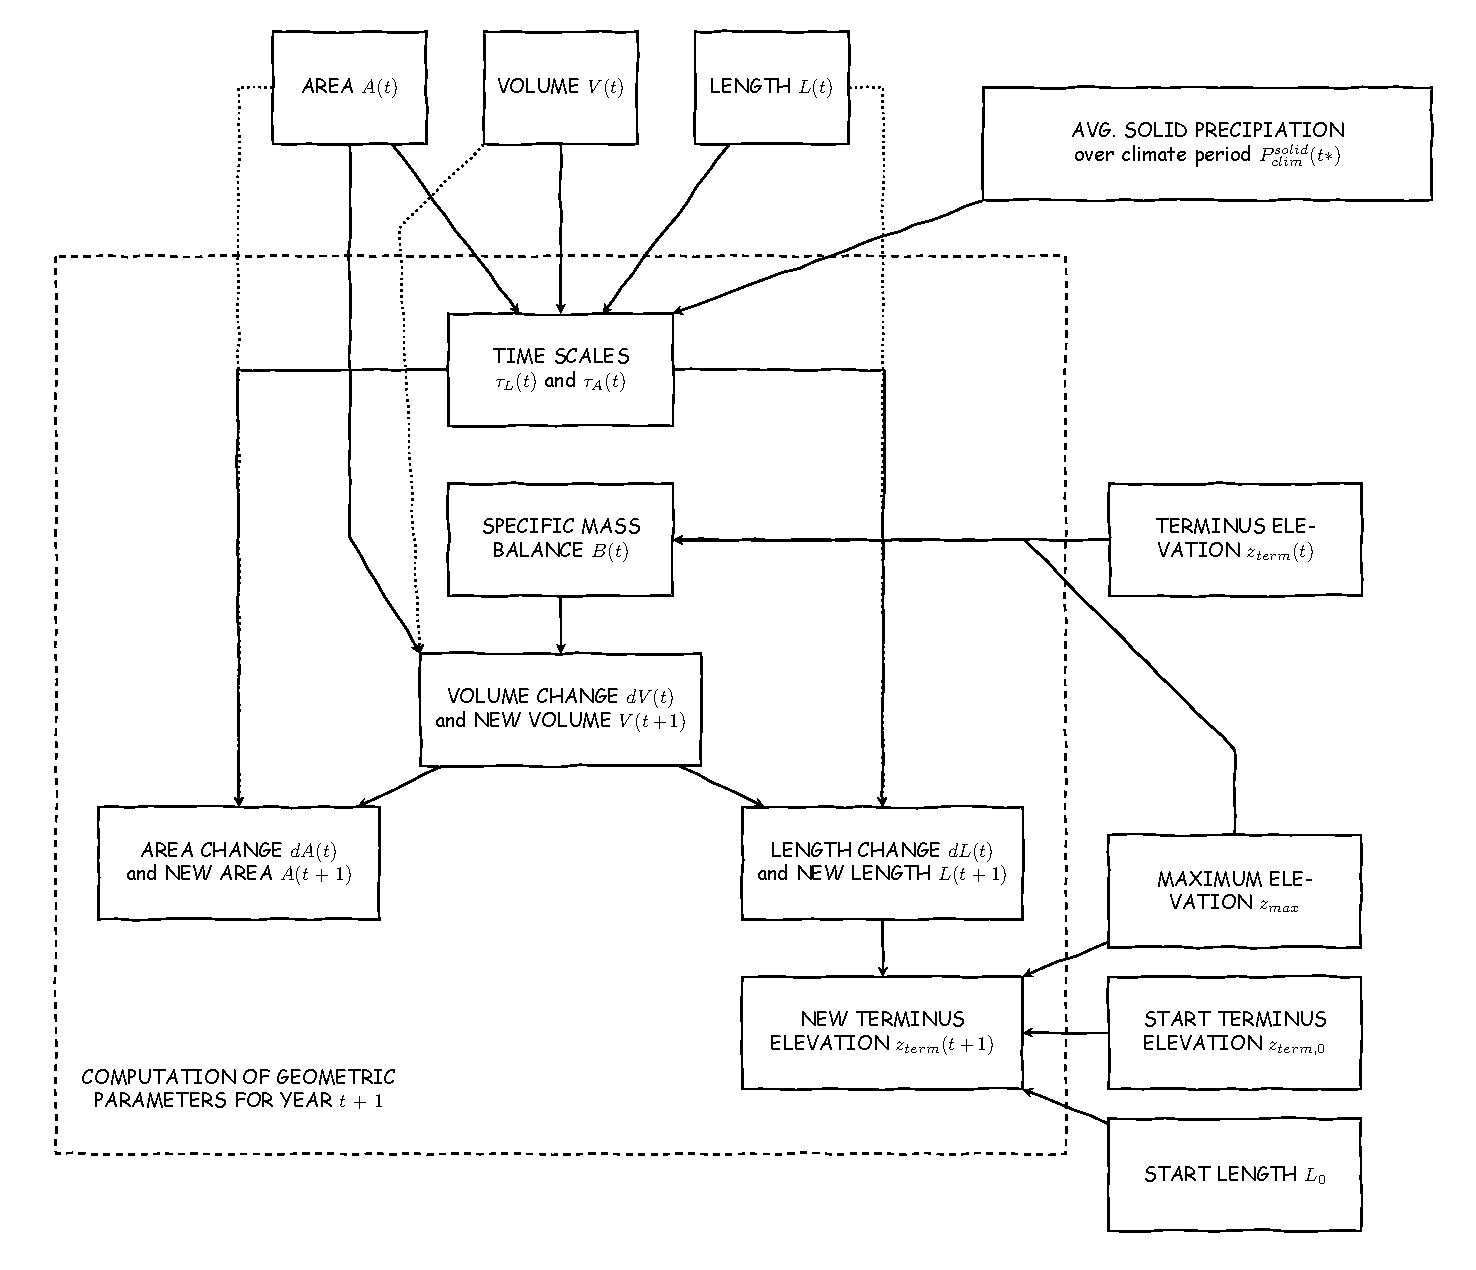
\includegraphics[width=\textwidth]{../flowchart/iterations/scaling.pdf}
            \caption{Schematic of the glacier evolution model's time stepping.}
            \label{fig:iteration-scheme}
        \end{figure}
        
        % Start area finding process ???
    
    % subsection glacier_evolution_model (end)

% section general_concepts (end)

% ==== SECTION 2 ===============================================================
\section{Implementation} % (fold)
\label{sec:implementation}

    \subsection{Mass balance models} % (fold)
    \label{sub:mass_balance_models_implementation}

        \subsubsection{Volume/area scaling mass balance model} % (fold)
        \label{ssub:volume_area_scaling_mass_balance_model_implementation}

            The \lstinline`VAScalingMassBalance` model is the implementation of the \textit{original} mass balance model by \citet{Marzeion2012b}. The model computes the mass balance of a glacier during the climate data period. The general concept is fairly similar to the \lstinline`oggm.core.massbalance.PastMassBalance` model. The main difference is, that the \vas{} mass balance model returns only one glacier wide average mass balance value, instead of point mass balance values for the different elevation bands.

            The mass balance model is initialized for a single glacier, denoted by the OGGM specific glacier directory \lstinline`gdir`. Per default, the model will use the calibrated mass balance parameters \mustar{} and \bias{} and read temperature and precipitation records from the preprocessed climate file \lstinline`climate_historical`. An alternative climate file can be used, by supplying either the filename and/or it's suffix via the parameters \lstinline`filename` and \lstinline`input_filesuffix`, repecitvely. It is possible to specify the start year and end year of the climate period (\lstinline`ys` and \lstinline`ye`), if not all available data should be used. The parameter \lstinline`repeat` controlls whether the climate period given by \lstinline`[ys, ye]` should be repeated indefinitely in a circular way.

            The \vas{} mass balance model inherits the following methods from the \lstinline`oggm.core.massbalance.MassBalanceModel` super class:
            \begin{itemize}
                \item \lstinline`get_annual_climate()` and \lstinline`get_monthly_climate()` compute and return the mass balance relevant climate information, i.e. positive air temperature at the terminus elevation in \si{\celsius} and solid precipitation amount in \si{\kg\per\square\m}, for the given year and month/year combination, respectively.
                \item \lstinline`get_annual_mb()` and \lstinline`get_monthly_mb()` compute and return the glacier wide average mass balance in \si{\m\per\s}, for the given year and month/year combination, respectively. The possible mass balance residual \bias{} is applied.
                \item \lstinline`get_specific_mb()` and \lstinline`get_monthly_specific_mb()` compute and return the glacier wide average specific mass balance in \si{mm w.e.\per yr}, for the given year and month/year combination, respectively. The possible mass balance residual \bias{} is applied.
            \end{itemize}
            All methods need the glacier terminus elevation \lstinline`min_hgt` and the maximal glacier surface elevation \lstinline`max_hgt` as parameters. The date is supplied via the \lstinline`year` parameter, using the hydrological float year convention. Given that the scaling mass balance model computes the glacier wide average mass balance, it is not possible to estimate the equilibrium line altitude. Hence, the the method \lstinline`get_ela()` is not implemented, in contrast to the \lstinline`PastMassBalance` model.
        
        % subsubsection volume_area_scaling_mass_balance_model_implementation (end)

        \subsubsection{Constant climate scenario} % (fold)
        \label{ssub:constant_climate_scenario_implementation}
            The \lstinline`ConstantMassBalance` model simulates a constant climate based on the observations averaged over a 31-year period centered on a given year \lstinline`y0`. Hence, the specific mass balance does not change from year to year. The task \lstinline`run_constant_climate(gdir, ...)` initializes a \lstinline`ConstantMassBalance` for the given glacier \lstinline`gdir` and runs for a given number of years \lstinline`nyears`. The task takes an additional temperature bias as parameters \lstinline`temp_bias`, to alter the observed climate records.

            The same idea of a constant climate is used during the mass balance calibration, solving the mass balance equation (Equation~\ref{eq:mass-balance}) for the temperature sensitivity \mustar. So per definition, \mustar{} is the temperature sensitivity to keep the glacier in equilibrium over the 31-year climate period centered around the \textit{equilibrium year} \tstar{} while neglecting a potential mass balance residual \bias. Consequentially, a \lstinline`ConstantMassBalance` model with \lstinline`y0` = \tstar{} keeps the glacier in equilibrium.
        
        % subsubsection constant_climate_scenario_implementation (end)

        \subsubsection{Random climate scenario} % (fold)
        \label{ssub:random_climate_scenario_implementation}

            Similar to the \lstinline`ConstantMassBalance` model, the \lstinline`RandomMassBalance` model is based on a 31-year period centered on a given year \lstinline`y0`. However, the mass balance years are randomly shuffled within that period. More precise, for each simulated year the model computes the specific mass balance using temperature and precipitation records from a randomly selected year within the given period. Hence, the model runs on a synthetic random climate scenario based on actual observations. A seed \lstinline`seed`' for the random generator can be supplied as parameter, to allow for reproducibility. Additionally, it is possible to choose between draws with and without replacement via the \lstinline`unique_sample` parameter.

            The task \lstinline`run_random_climate(gdir, ...)` works analogously to the task \lstinline`run_constant_climate(gdir, ...)`, using an instance of \lstinline`RandomMassBalance` model instead of the \lstinline`ConstantMassBalance` model. Hence, using the climatological period centered around \lstinline`y0` = \tstar, the model glacier should stay in an equilibrium state while underlying minor fluctuations. Supplying a positive or negative temperature bias will result in a retreating or advancing model glacier, respectively, reaching a new equilibrium after some years.
        
        % subsubsection random_climate_scenario_implementation (end)
    
    % subsection mass_balance_models_implementation (end)

    \subsection{Glacier evolution model} % (fold)
    \label{sub:glacier_evolution_model_implementation}

        The \lstinline`oggm-vas.VAScalingModel` is the implementation of the above describe glacier evolution model (see Section~\ref{sub:glacier_evolution_model}, \citet[cf.]{Marzeion2012b}) into the OGGM framework. The full source code is publicly available on \href{https://github.com/OGGM/oggm-vas}{GitHub}.

        An instance of the \lstinline`oggm-vas.VAScalingModel` class is initialized with the initial area \lstinline`area_m2_0`, the initial glacier terminus elevation \lstinline`min_hgt` and maximum glacier surface elevation \lstinline`max_hgt` and an instance of a \lstinline`oggm-vas.VAScalingMassBalance` model. Additionally, the start year of the simulation \lstinline`year_0` must be defined. Those initial values are stored as instance variables, since they are needed for later computations. Other than that, the \lstinline`oggm-vas.VAScalingModel` object stores all model parameters as instance variables for the current year it is in. This includes glacier geometries ($V$, $A$, $L$, $z_\text{min}$, $z_\text{max}$) and their changes ($\Delta V$, $\Delta A$, $\Delta L$), time scales ($\tau_A$, $\tau_L$), the mass balance model and the specific mass balance $B$, but also constants like the scaling parameters ($c_A$, $\gamma$, $c_L$, $q$) and ice density $\rho_\text{ice}$.

        To advance the glacier model, there are three different methods. The \lstinline`step()` method advances the model by one year, following the above described steps (see Section~\ref{sub:glacier_evolution_model}). The method \lstinline`run_until(year_end)` runs the model until the specified year and returns the geometric glacier parameters at the end of the model evolution (year, length, area, volume, terminus elevation and specific mass balance). Thereby, the model starts from whatever year it currently is in. It is possible to start the model run from \lstinline`year_0` with the flag \lstinline`reset`. The method \lstinline`run_until_and_store()` works analagous to the previous one, with the difference that all parameters are stored for each time step (i.e., for each year). The resulting data set is returned and possible stored to file, if a file path is give. The method \lstinline`run_until_equilibrium()` tries to run the glacier model until an equilibrium state is reached. The model runs for a fixed number of iteratrions \lstinline`max_ite`, the total elapsed time changes with the chosen time step \lstinline`ystep`. The iteration breaks, either if the glacier volume is below \SI{1}{\cubic\meter} or an equilibirum is reached. An equilibrium state is reached, if the volume change rate $|V(t) - V(t+\Delta t)|/V(t)$ falls below a given value \lstinline`rate`. Therefore, the method can only be used with a \hyperref[ssub:constant_climate_scenario_implementation]{constant climate scenario} (see Section~\ref{sub:mass_balance_models_implementation}).
    
    % subsection glacier_evolution_model_implementation (end)

% section implementation (end)


% ==== SECTION 3 ===============================================================
\section{Experimental setup} % (fold)
\label{sec:experimental_setup}
    
    % intro
    Implementing the \vas{} model is all good and well, but how does it compare to the flowline model?!
    While successfully passing the unit test is a necessity---or at least good programming practice---unit tests are only testing for coding errors and not for the physicality of the results. Nor do they answer the main research question: ``What information is gained from the use of a physical based flowline model?'' The following experiments run the newly implemented model in a variety of setting and compare it to the OGGM flowline model. The focus is on the intrinsic model behavior and its comparison to the flowline model, not on absolute ice volume estimations.

    The experiments start on the smallest scale possible, namely with a single glacier. This first test case is intended to get a feel for the model and set the stage for the following experiments. Qualitative conclusions are drawn from time series of glacier geometries in response to different equilibrium climates. Some more quantitative results are obtained from an analysis of autocorrelation function and power spectral density of length change signals under a white noise climate, inspired by \citep{Roe2014}. Both analyses can only be performed on the signal of a single glacier, since mirroring oscillation of different glaciers could cancel each other out. To avoid another N-of-1 experiment, six different Alpine glaciers are investigated during this step. 
    While it may be necessary for the aforementioned experiments, it is not appropriate to apply scaling relations to a single glacier. \Vas{} should only be applied to a collection of glaciers \citep{Bahr2015}. The first regional run looks at the evolution of aggregate ice volume of all Alpine glaciers for different equilibrium climate scenarios.
    Any differences between the \vas{} model and the flowline model found above may be caused by the parameters defining the scaling relations. The parameters in question are the length timescale and area timescale for the response time scaling as well as the scaling constants and scaling exponents for the volume/length and \vas{}. A sensitivity analysis of said parameters is performed on a single glacier and on the collective Alpine glaciers.
    As a final experiment, the \vas{} model is used to estimate the potential ice melt over the coming one-hundred years for all Alpine glaciers. This is done by using todays climate in combination with a different positive temperature biases to simulate different climate scenarios.

    All the aforementioned experiments can be classified as equilibrium experiments. As most things in nature, glaciers strive toward an equilibrium condition. Such an equilibrium is reached eventually, by adjusting the glacier's geometry in reaction to changes in climatic conditions. Analyzing the behavior of a glacier model subjected to a step change in climate can be used to get insight into the dynamics of the numerical model, e.g. to estimate response times. The OGGM provides two convenient climate scenarios (or rather mass balance models) for such equilibrium experiment: the \lstinline`ConstantMassBalance` model and the \lstinline`RandomMassBalance` model. The implementation and workings of both mass balance models are described in Section~\ref{sub:mass_balance_models_implementation} (see \hyperref[ssub:constant_climate_scenario_implementation]{constant} and \hyperref[ssub:random_climate_scenario_implementation]{random} climate scenario). The hereafter detailed experiments use the HISTALP dataset \citep{Auer2007} as climate input data, with the corresponding hyper parameters (see  \href{https://oggm.org/2018/08/10/histalp-parameters/}{Mass-balance model calibration for the Alps} \citep{Dusch2018} on the OGGM blog for more information). This obviously limits the suitable glaciers to the ones inside the HISTALP domain, i.e. the Alps. The HISTALP domain corresponds to the region 11-01 of the Randolph Glacier Inventory (RGI) \citep{RGI2017,Pfeffer2014} (version 6.x) and lists 3892 glaciers.

    The following paragraph briefly lists the preprocessing tasks needed for the equilibrium runs. For a detailed description of OGGM workflow see \citet{Maussion2019} and the \href{https://docs.oggm.org}{OGGM documentation}.
    \begin{description}[noitemsep]
        \item[GIS tasks:] using the digital elevation model (DEM) from the Shuttle Radar Topography Mission (\href{http://srtm.csi.cgiar.org/}{SRTM}, \citet{Jarvis2008}) and the RGI glacier outlines to compute a local grid, compute a glacier mask, compute centerlines and corresponding catchment areas;
        \item[climate tasks:] extract the HISTALP time series for the grid point nearest to the glacier and write it in the \lstinline`climate_historical.nc` file;
        \item[mass balance calibration:] computing the glacier specific mass balance parameters \tstar{}, \mustar{} and \bias{};
        \item[inversion tasks:] running the ice thickness inversion to estimate the bed topography (needed only for the flowline model);
    \end{description}

    The actual model runs are invoked via the \lstinline`run_constant_climate` and \lstinline`run_random_climate` tasks (see Section~\ref{sub:mass_balance_models_implementation} for implementation details). The used settings depend on the intended experiment and are detailed in the following sections.

    \subsection{Single glacier test case} % (fold)
    \label{sub:single_glacier_test_case_setup}

        The first qualitative look at the \vas{} performance uses the Hintereisferner (RGI60-11.00897) as test case. This test case is intended to get a feel for the \vas{} model and set the stage for the following experiments, by comparing the two mass balance models suitable for equilibrium experiments.
        It has to be noted that \vas{} applied to single glaciers gives only an order of magnitude estimation. The scaling constant $c$ is a globally averaged value, and the relative error in scaling constant is directly proportional to the error in estimated ice volume \citep{Bahr2015}. However, a qualitative comparison between the \vas{} model and the flowline model is more practicable and meaningful for a single glacier. The model's sensitivity to its scaling parameters is investigated in Section~\ref{sec:sensitivity_experiments_results}

        % Mass balance calibration and mass balance models using the same tstar
        For this first experiment, both evolution models run with the \lstinline`ConstantMassBalance` model and the \lstinline`RandomMassBalance` model, for 1000 years each. Both mass balance models emulate an equilibrium climate to keep the glacier in its initial equilibrium state. Therefore, the mass balance models must be initialized with the climatic period centered around the equilibrium year, i.e., \lstinline`y0` = \tstar{}. As explained above, the mass balance calibration depends, among others, on the chosen \tstar{} (Section~\ref{sub:temperature_index_model}, see \hyperref[ssub:mb_calib]{Calibration of the mass balance parameters}). Hence, to run both evolution models with the identical climatic forcing, \tstar{} must be equal for both. This is done by computing the temperature sensitivity \mustar{} for both models using the same \tstar{} reference table (\lstinline`oggm_ref_tstars_rgi6_histalp.csv`, corresponding to the flowline model). Additionally, the mass balance residual must be omitted during the model run ($\beta^*$ = 0, as per the definition of \mustar{}, see Section~\ref{sub:temperature_index_model}). Each mass balance model runs three different climate scenarios defined by the temperature biases of \SI{0}{\celsius}, \SI{-0.5}{\celsius} and \SI{+0.5}{\celsius}. These runs will be referred to as \emph{equilibrium run}, run with \emph{positive mass balance bias} and run with \emph{negative mass balance bias}, respectively.
    
    % subsection single_glacier_test_case_setup (end)

    \subsection{Autocorrelation function and Power spectral density} % (fold)
    \label{sub:autocorrelation_and_power_spectral_density_setup}

        The correlation is a measure for the linear dependency between two (random) variables. A positive correlation coefficient close to +1 indicates a strong direct relationship between two variables, while a negative correlation coefficient close to -1 indicates a strong indirect relationship between two variables. A correlation coefficient around zero indicates that the variables are independent. The autocorrelation function (ACF) computes the correlation coefficient between a signal and a lagged copy of itself as a function of lag time $k$. A lagged copy of a signal is simply the signal shifted by time $k$. The intuition behind the ACF is the relation between past and present values of a signal. It is used find possible periodicities hidden in noisy signals and gives an estimate on how strong neighboring data points influence each other. A high autocorrelation at lag time $k$ indicates that data points that are a time $k$ apart have similar values. The ACF at lag time $k=0$ is obviously one, since any signal correlates to \SI{100}{\percent} with itself. The partial autocorrelation function (PACF) measures only the direct influence of values with lag time $k$, eliminating the effects of all shorter lag times \citep{BoxJenkins2015}. Plots of both functions give a qualitative insight...

        On of the simples models to describe a stationary random time series is an autoregressive-moving-average (ARMA) model. It predicts future values of a random variable based on a linear combination of past values and past error terms of said variable. The number of included lag terms is defined by the order $p$ of the autoregressive term and the order $q$ of the moving-average term. The number of statistically significant non-zero terms of the ACF and PACF can be used to estimate the order $q$ and $p$ of an ARMA(p,q) model, respectively \citep{BoxJenkins2015}. The three stage model by \citet{Roe2014} is an ARMA(3,3) model. While the goal of this work is not to define an ARMA glacier model, a brief analysis is provided in an attempt to quantify the autocorrelation.
        
        The power spectral density (PSD) is the Fourier transform of the ACF. A Fourier transform decomposes a signal into a spectrum of frequencies, or much rather into a collection of frequency bins for the discrete Fourier transform used. Hence, the PSD is as function of frequency. The signal's power describes its energy per unit time. Thereby, the power is of unit \si{[X^2]} if the signal's unit is \si{[X]} and must not be actual physical power of unit \si{[\watt]}. The power density is the power normalized with the frequency bin width, hence the power density has the unit \si{[X^2/\hertz]} if the frequency is measured in \si{[\hertz]}. The PSD is used to find dominant frequencies in noisy signals.

        The ACF, PACF and PSD are computed for the glacier length signal, in analogy to \citep{Roe2014}. To avoid another N-of-1 experiment, the behavior of the \vas{} model is compared to the flowline model for the following six Alpine glaciers:
        \begin{itemize}
            \item Hintereisferner (RGI60-11.00897), Ötztal Alps, Austria
            \item Pasterze (RGI60-11.00106), Hohe Tauern, Austria
            \item Mer de Glace (RGI60-11.03643), Mont Blanc massif, France
            \item Glacier d'Argentière (RGI60-11.03638), Mont Blanc massif, France
            \item Großer Aletschgletscher (RGI60-11.01450), Bernese Alps, Switzerland
            \item Rhonegletscher (RGI60-11.01238), Urner Alps, Switzerland
        \end{itemize}
        These glaciers are selected because of their size and notoriety, however the choice is somewhat arbitrary. All glaciers are subjected to different random (white noise) climate conditions for 23\ 000 years. The remaining settings are analogous to the single glacier test case. The \lstinline`RandomMassBalance` model is initialized around the respective \textit{equilibrium year} for each glacier (\lstinline`y0` = \tstar), whereby both evolution model use the same \tstar{} reference table. The mass balance residual is omitted ($\beta^* = 0$). The input climate shows no autocorrelation and a constant PSD curve and can therefore be classified as white noise with non-zero mean.
        To increase the amount of available data, each glacier is subjected to three different climate scenarios, specified by a temperature bias of \SI{-0.5}{\celsius}, \SI{0}{\celsius} and \SI{+0.5}{\celsius}. The initial 3000 years during which the glaciers adjust to the changed climate are clipped, which leaves three different sizes of the same glacier, each in equilibrium condition. An ARMA model can only be applied to stationary time series. Stationarity is given if the mean and the variance are time independent and the signal shows no seasonality (for a formal definition \citet[e.g.,][]{BoxJenkins2015}). While the stationarity is easily determined manually for the glacier length signals, an Augmented Dickey--Fuller test (\href{https://www.statsmodels.org/devel/generated/statsmodels.tsa.stattools.adfuller.html}{\lstinline`statsmodels.tsa.stattools.adfuller`}, \citet{Cheung1995-ADFuller}) results in $p$-values far below \SI{1}{\percent} for all signals.

        The ACF is computed using the python function \href{https://www.statsmodels.org/devel/generated/statsmodels.tsa.stattools.acf.html}{\lstinline`statsmodels.tsa.stattools.acf`} via a fast Fourier transform. The PSD is estimated using Welch's method. Welch's method reduces the variance in  estimated power density by time-averaging, at the cost of frequency resolution \citep[e.g.,][]{Welch1967, Proakis2007}.  The remaining 20\ 000 data points are divided into nineteen time windows with a size of 2000 data points and a \SI{50}{\percent} overlap. The windows are tapered using the Hann function. For details about additional parameters see the default values of the python function \href{https://docs.scipy.org/doc/scipy/reference/generated/scipy.signal.welch.html}{\lstinline`scipy.signal.welch`}, which is used for the PSD computation.
    
    % subsection autocorrelation_fand_power_spectral_density_setup (end)

    \subsection{Regional runs with all Alpine glaciers} % (fold)
    \label{sub:regional_runs_with_all_alpine_glaciers_setup}
        \Vas{} applied to single glaciers gives only an order of magnitude estimation, since the scaling constant $c$ is a globally averaged value. A potential relative error in $c$ will be directly transfered to any volume estimation. Hence, \vas{} should only be applied to collections of glaciers \citep{Bahr2015}. 
        This first regional simulations over all Alpine glaciers are based on an equilibrium climate, in analogy to the single glacier test case.

        These simulations are intended to reflect the reality as good as possible. Hence, the default OGGM \hyperref[ssub:mb_calib]{mass balance calibration} is used (see Section~\ref{sub:temperature_index_model}). This means, each evolution model uses its own \tstar{} reference table (which may result in different \tstar{} for the same glacier depending on the evolution model) and the mass balance residual \bias{} is used for each run. Both evolution models run with the \lstinline`ConstantMassBalance` model and the \lstinline`RandomMassBalance` model, for 1000 years each. The mass balance models are initialized with \lstinline`y0` = \tstar{} and run with the same three different temperature biases as before (\SI{0}{\celsius}, \SI{-0.5}{\celsius}, \SI{+0.5}{\celsius}).
    
    % subsection regional_runs_with_all_alpine_glaciers_setup (end)

    \subsection{Sensitivity experiments} % (fold)
    \label{sub:sensitivity_experiments_setup}
        % introduction
        ... Before moving to the final experiments estimating future ice volume loss, it is necessary to determine the model's sensitivities. The following sensitivity analysis investigates the effects of the model-internal time scales and scaling parameters on the model behavior. Both parameter sets are specific to the scaling model, since they determine the response time scaling as well as the volume/length and \vas{}. For consistency, the sensitivity experiments are performed on Hintereisferner (RGI60-11.00897) as a single glacier test case and on all Alpine glaciers inside the HISTALP domain. For simplicity, only the \lstinline`ConstantMassBalance` model with a temperature bias of \SI{+0.5}{\celsius} is used for all runs.

        % Time scales
        The scaling model estimates glacial evolution via the implemented response time scaling. Response time scaling adjusts the yearly change in geometry in relation to the total possible change using the model-internal response time scales for length and area, $\tau_L$ and  $\tau_A$, respectively (see Section~\ref{sub:glacier_evolution_model} and \ref{sub:glacier_evolution_model_implementation} for details).
        However, the model-internal time scales are only a rough estimate and hence good possible tuning parameters. The sensitivity experiments compare the model output for different time scales, modified by a linear factor $\tau_\text{sens.} = f \cdot \tau$. Hereby, the factor $f$ is only applied to $\tau_L$, since $\tau_A$ is a linear function of $\tau_L$. The default values with $f=1$ serves as baseline. From there, the model-internal time scales are halved ($f=0.5$) and doubled ($f=2$). 

        % Scaling parameters
        The other obvious choice of tuning parameters are the scaling exponents and scaling constants. The scaling constants for volume/length and \vas{}, $c_L$ and $c_A$, respectively, can be seen as random variables. The randomness stems from the statistically similar but not identical dimensionless parameters for length, area and volume  varying from glacier to glacier. Thanks to the law of large numbers, the global scaling constants $c_L = \SI{0.0180}{\kilo\meter^{3-q}}$ and $c_A = \SI{0.0340}{\kilo\meter^{3-2\gamma}}$ are a reasonable choice for a global ice volume estimation \citep{Bahr2015}. However, those parameters may be a bad fit for certain regions and therefore need calibration.
        While the scaling constants are not constant, the scaling exponents are. The \vas{} exponent was first derived as the slope of the linear regression of volume and area observations in log-log space \citep[e.g.,][]{Chen1990}. \citet{Bahr1997b} found that their values are fixed by the underlying physics and depend only on a single set of closure conditions. The closure conditions are in turn tightly bound by observations and different common closures lead to the same results. Hence, it is strongly advised to use the global values of $q = 2.2$ and $\gamma = 1.375$  for the volume/length and \vas{}. Additionally, even with different closure conditions could be justified, the area scaling exponent is bound $1.1\dot{6} \leq \gamma \leq 1.5$ by simple geometric reasoning \citep[Section 8.2]{Bahr2015}. 

        As for the time scale sensitivity experiments, the global values of the scaling exponents serve as baseline. The next run uses custom scaling constant derived from a linear regression in log-log space but with a fixed slope corresponding to the global scaling exponents. The last run uses full custom scaling constants and exponents, again derived from a linear regression in log-log space. For reasons of simplicity, data points of volume, area and length are taken from the OGGM flowline model glaciers and not from observations. The inversion volume serves as glacier volume, the RGI area as surface area and the longest centerline as glacier length.
        
        Since a linear regression can not be computed from a single data point, the Hintereisferner test case differentiates only between global and custom scaling constants (obtained by solving the scaling relations for $c$) while using the global default scaling exponents. The following two sets of scaling parameters are used:
        \begin{enumerate}[label=(\alph*)]
            \item global (default) values of $c_L = \SI{4.551}{\meter^{3-q}}$, $q = 2.2$ for volume/length scaling and $c_A = \SI{0.191}{\meter^{3-2\gamma}}$, $\gamma = 1.375$ for \vas{}
            \item custom scaling constants $c_L = \SI{1.555}{\meter^{3-q}}$ and $c_A = \SI{0.252}{\meter^{3-2\gamma}}$ with the global and physically based scaling exponents $q = 2.2$ and $\gamma = 1.375$
        \end{enumerate}
        For comparability, the sensitivity runs on Hintereisferner (RGI60-11.00897) are setup exactly the same as the test case (see Section~\ref{sub:single_glacier_test_case_setup}). This means a fixed \textit{equilibrium year} $t^{*} = 1927$ and no mass balance residual during the run. The regional Alpine runs are setup as before (see Section~\ref{sub:regional_runs_with_all_alpine_glaciers_setup}) and use the following three sets of scaling parameters:
        \begin{enumerate}[label=(\alph*)]
            \item global (default) values of $c_L = \SI{4.551}{\meter^{3-q}}$, $q = 2.2$ for volume/length scaling and $c_A = \SI{0.191}{\meter^{3-2\gamma}}$, $\gamma = 1.375$ for \vas{}
            \item custom scaling constants $c_L = \SI{1.805}{\meter^{3-q}}$ and $c_A = \SI{0.250}{\meter^{3-2\gamma}}$ with the global and physically based scaling exponents $q = 2.2$ and $\gamma = 1.375$
            \item custom scaling constants and scaling exponents $c_L = \SI{0.244}{\meter^{3-q}}$, $q = 2.517$ for volume/length scaling and $c_A = \SI{0.117}{\meter^{3-2\gamma}}$, $\gamma = 1.441$ for \vas{}
        \end{enumerate}

        Disclaimer: As already mentioned, this work is focused on the model behavior much rather than an absolute ice volume estimation. While scaling constants and exponents based in observations would be preferable, the values of the custom scaling parameters are less important as long as the are different from the global values. In fact, the sensitivity experiment could easily be conducted with a set of fabricated exponents. For the same reason, it is inconsequential that scaling exponents derived from a numerical model may differ depending on the model's closure conditions \citep[Section 8.9]{Bahr2015}. It is hereby noted that this potential source for errors is acknowledged, and the flowline model is not tested for its closure conditions. While the custom scaling exponents lie within the range of physical sensible values, finding closure conditions supporting the computed values would go (far) beyond the scope of this work.

    % subsection sensitivity_experiments_setup (end)

    \subsection{Commitment runs} % (fold)
    \label{sub:commitment_runs_setup}
        One of the easiest ways of estimating future glacial evolution are so called \textit{commitment runs}.
        The name stems from the \textit{commitment} to a given climate, which is then held constant for the entire run. For example, applying the current climate to the current glaciers for the next, say, 100 years, would give a---naively optimistic---lower bound of the expected glacial retreat. As for the first regional run, ... % TODO

        While a climate scenario with yearly fluctuations is more physical than a completely constant climate, the resulting ice volume changes are comparable (see Section~\ref{sub:time_series_results}). Which is why, the following experiments can be limited to the \lstinline`ConstantMassBalance` model without any loss of information. For a more tangible experiment, the \lstinline`ConstantMassBalance` model is initialized with todays climate. Todays climate is assumed to be the average over the most recent 31 years. For the HISTALP dataset this corresponds to the period from 1984 to 2014 with \lstinline`y0 = 1999`. Since we live in a period of global warming, additional positive temperature biases of \SI{0}{\celsius}, \SI{+0.5}{\celsius} and \SI{+1.5}{\celsius} are used. Again, the default OGGM \hyperref[ssub:mb_calib]{mass balance calibration} is used assuring the most physical outcome.
    
    % subsection commitment_runs_setup (end)

% section experimental_setup (end)